\section{Diseño de software} \label{sec:dis}
% (estático e dinámico) ou do hardware: indicaranse os aspectos máis relevantes correspondentes ao deseño do traballo realizado
% estatico -> diagrama de clases
% dinamico -> diagrama de secuencia

    En esta sección se detallan los aspectos más importantes sobre el diseño del software estático y dinámico que se han llevado a cabo en este proyecto.
    
    Tal y como se refleja en la figura \ref{fig:class-diagram}, se puede apreciar el diagrama de clases que corresponde al \textit{Agente}. Dicho diagrama permite tener una visión global de cómo se relacionan entre sí las clases que componen el sistema, mostrando sus atributos, propiedades y funciones.
    
    Además de lo antes mencionado, en las figuras \ref{fig:sequence-diagram-service} y \ref{fig:sequence-diagram-cli} se muestran dos diagramas de secuencia detallados, estos indican las acciones efectuadas durante los procesos de obtención y utilización de la información por parte de los \textit{plugins}, en ejecuciones como servicio y como usuario interactivo.

    \begin{figure}[h!]
    \centering
        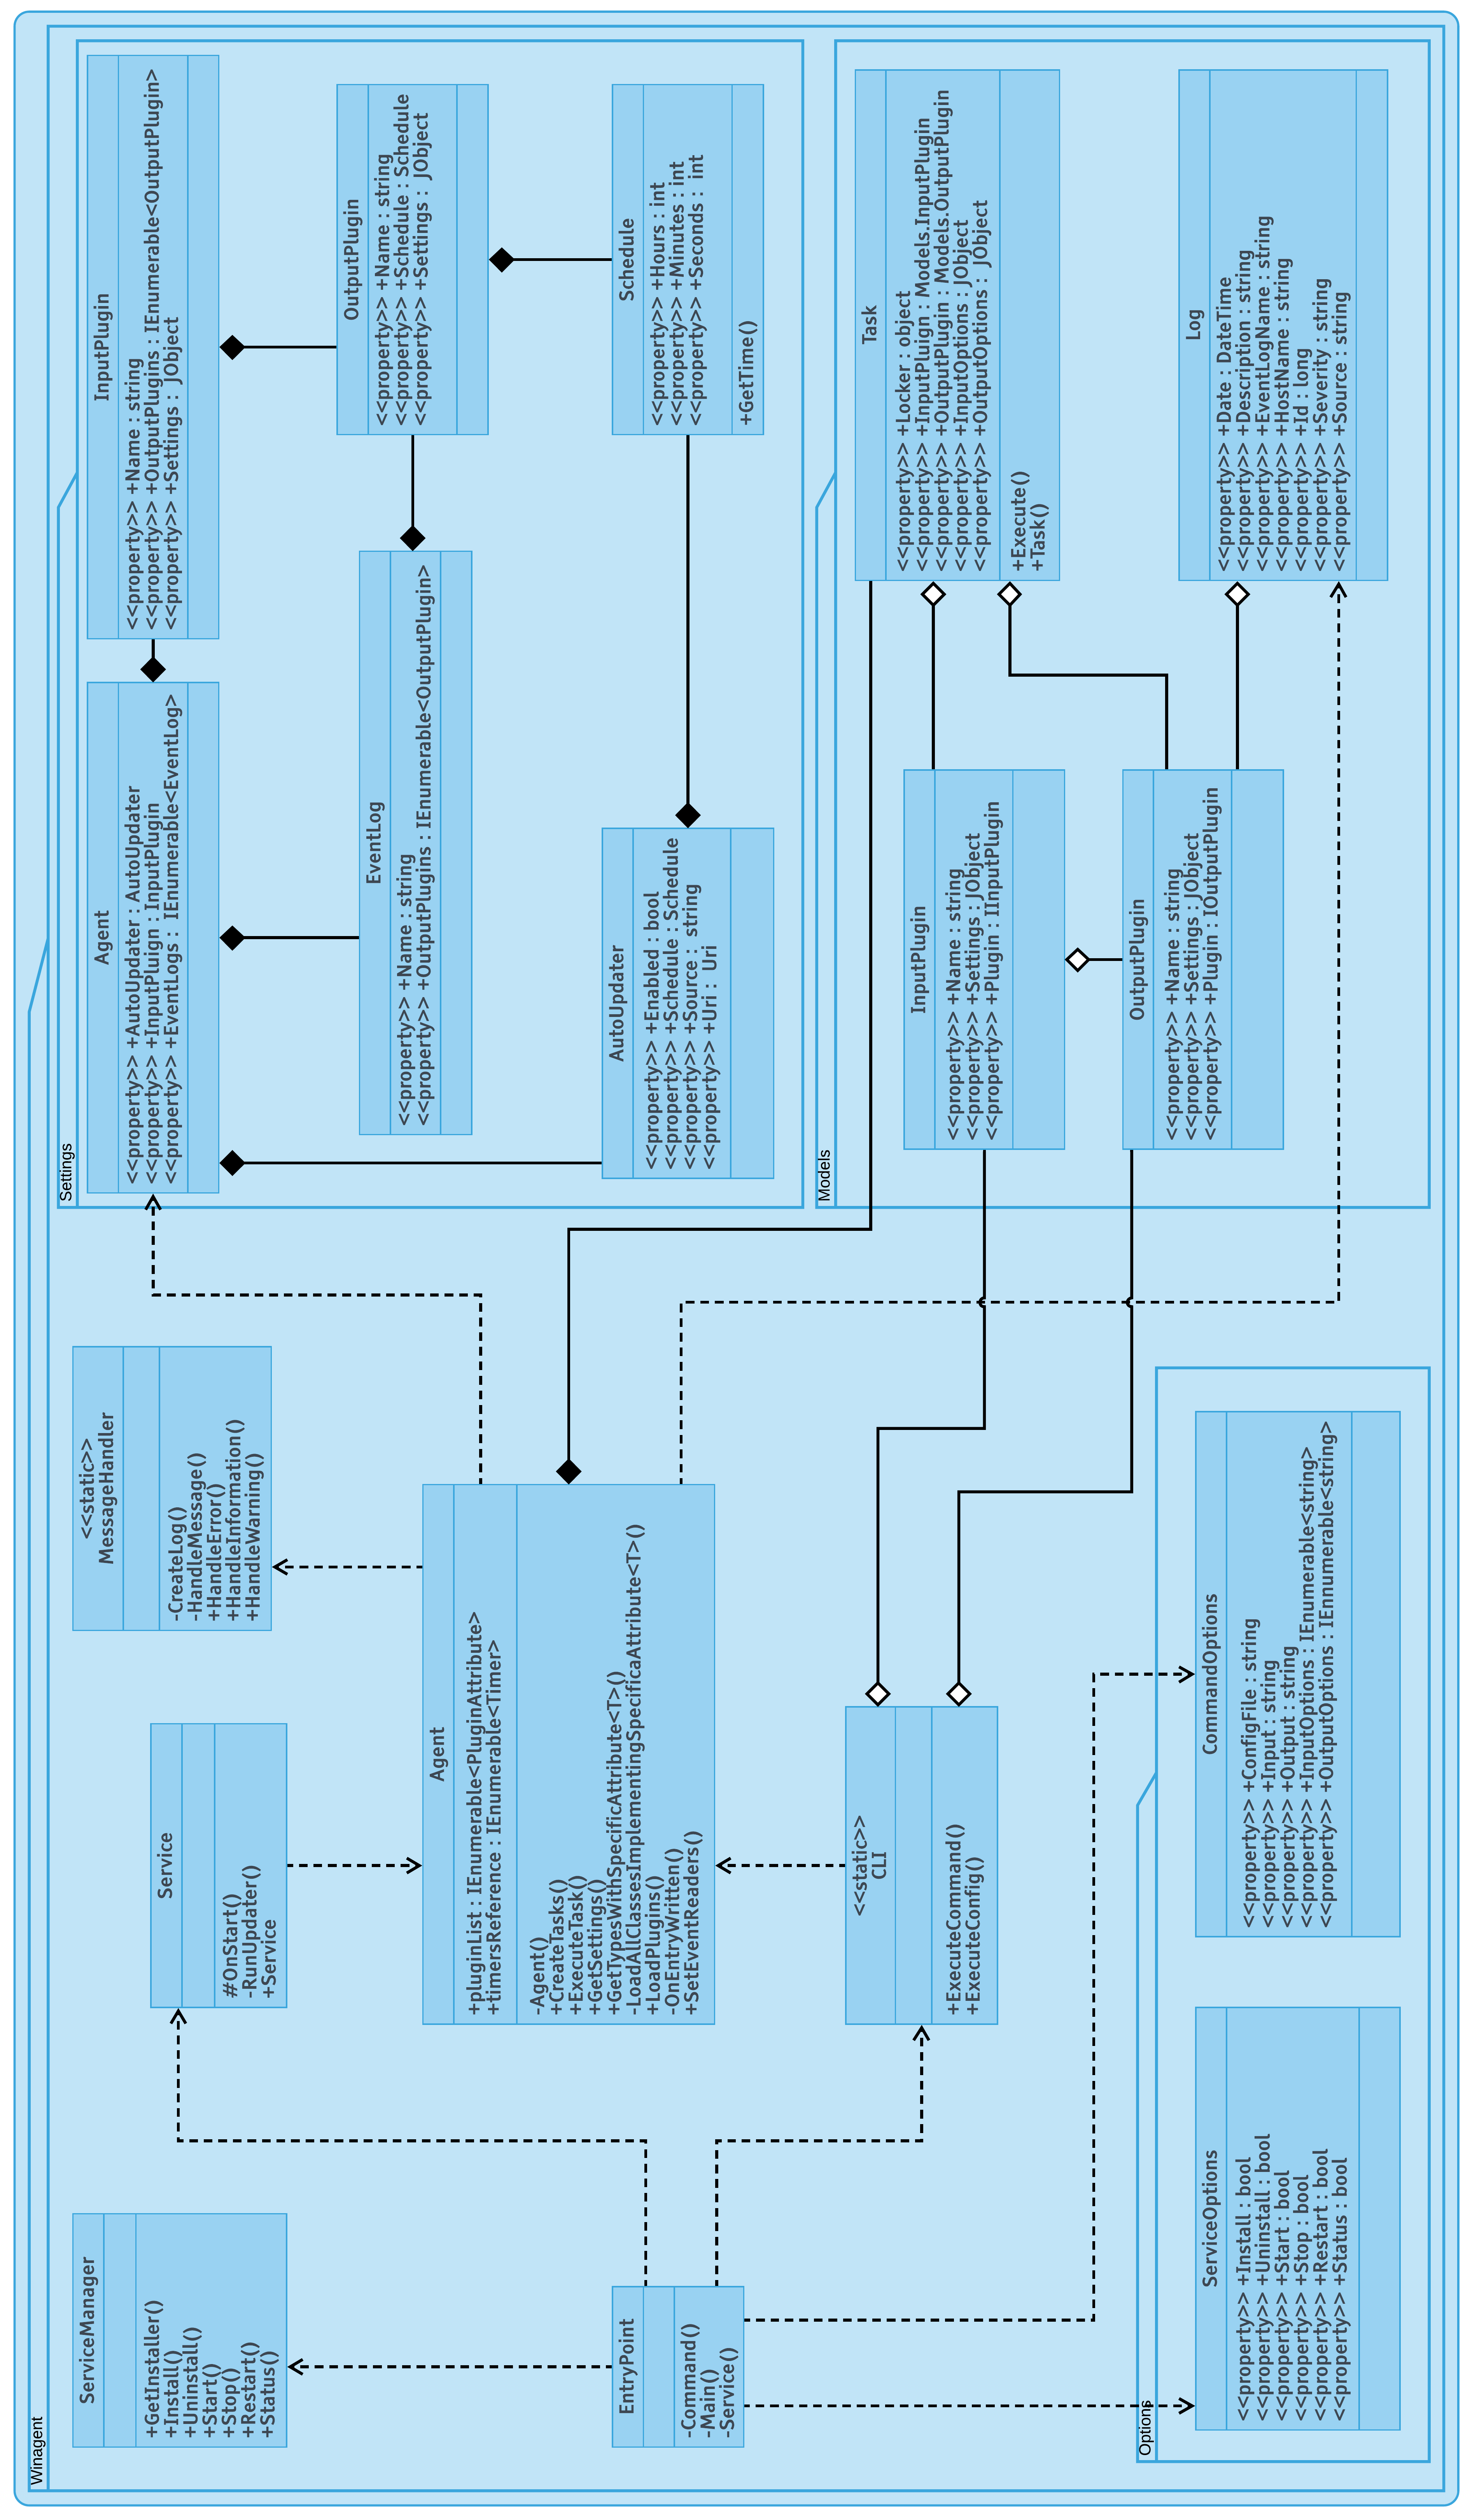
\includegraphics[scale=0.138]{diagrama-de-clases.png}
        \caption{Diagrama de clases}
        \label{fig:class-diagram}
    \end{figure}

    \begin{figure}[h!]
    \centering
        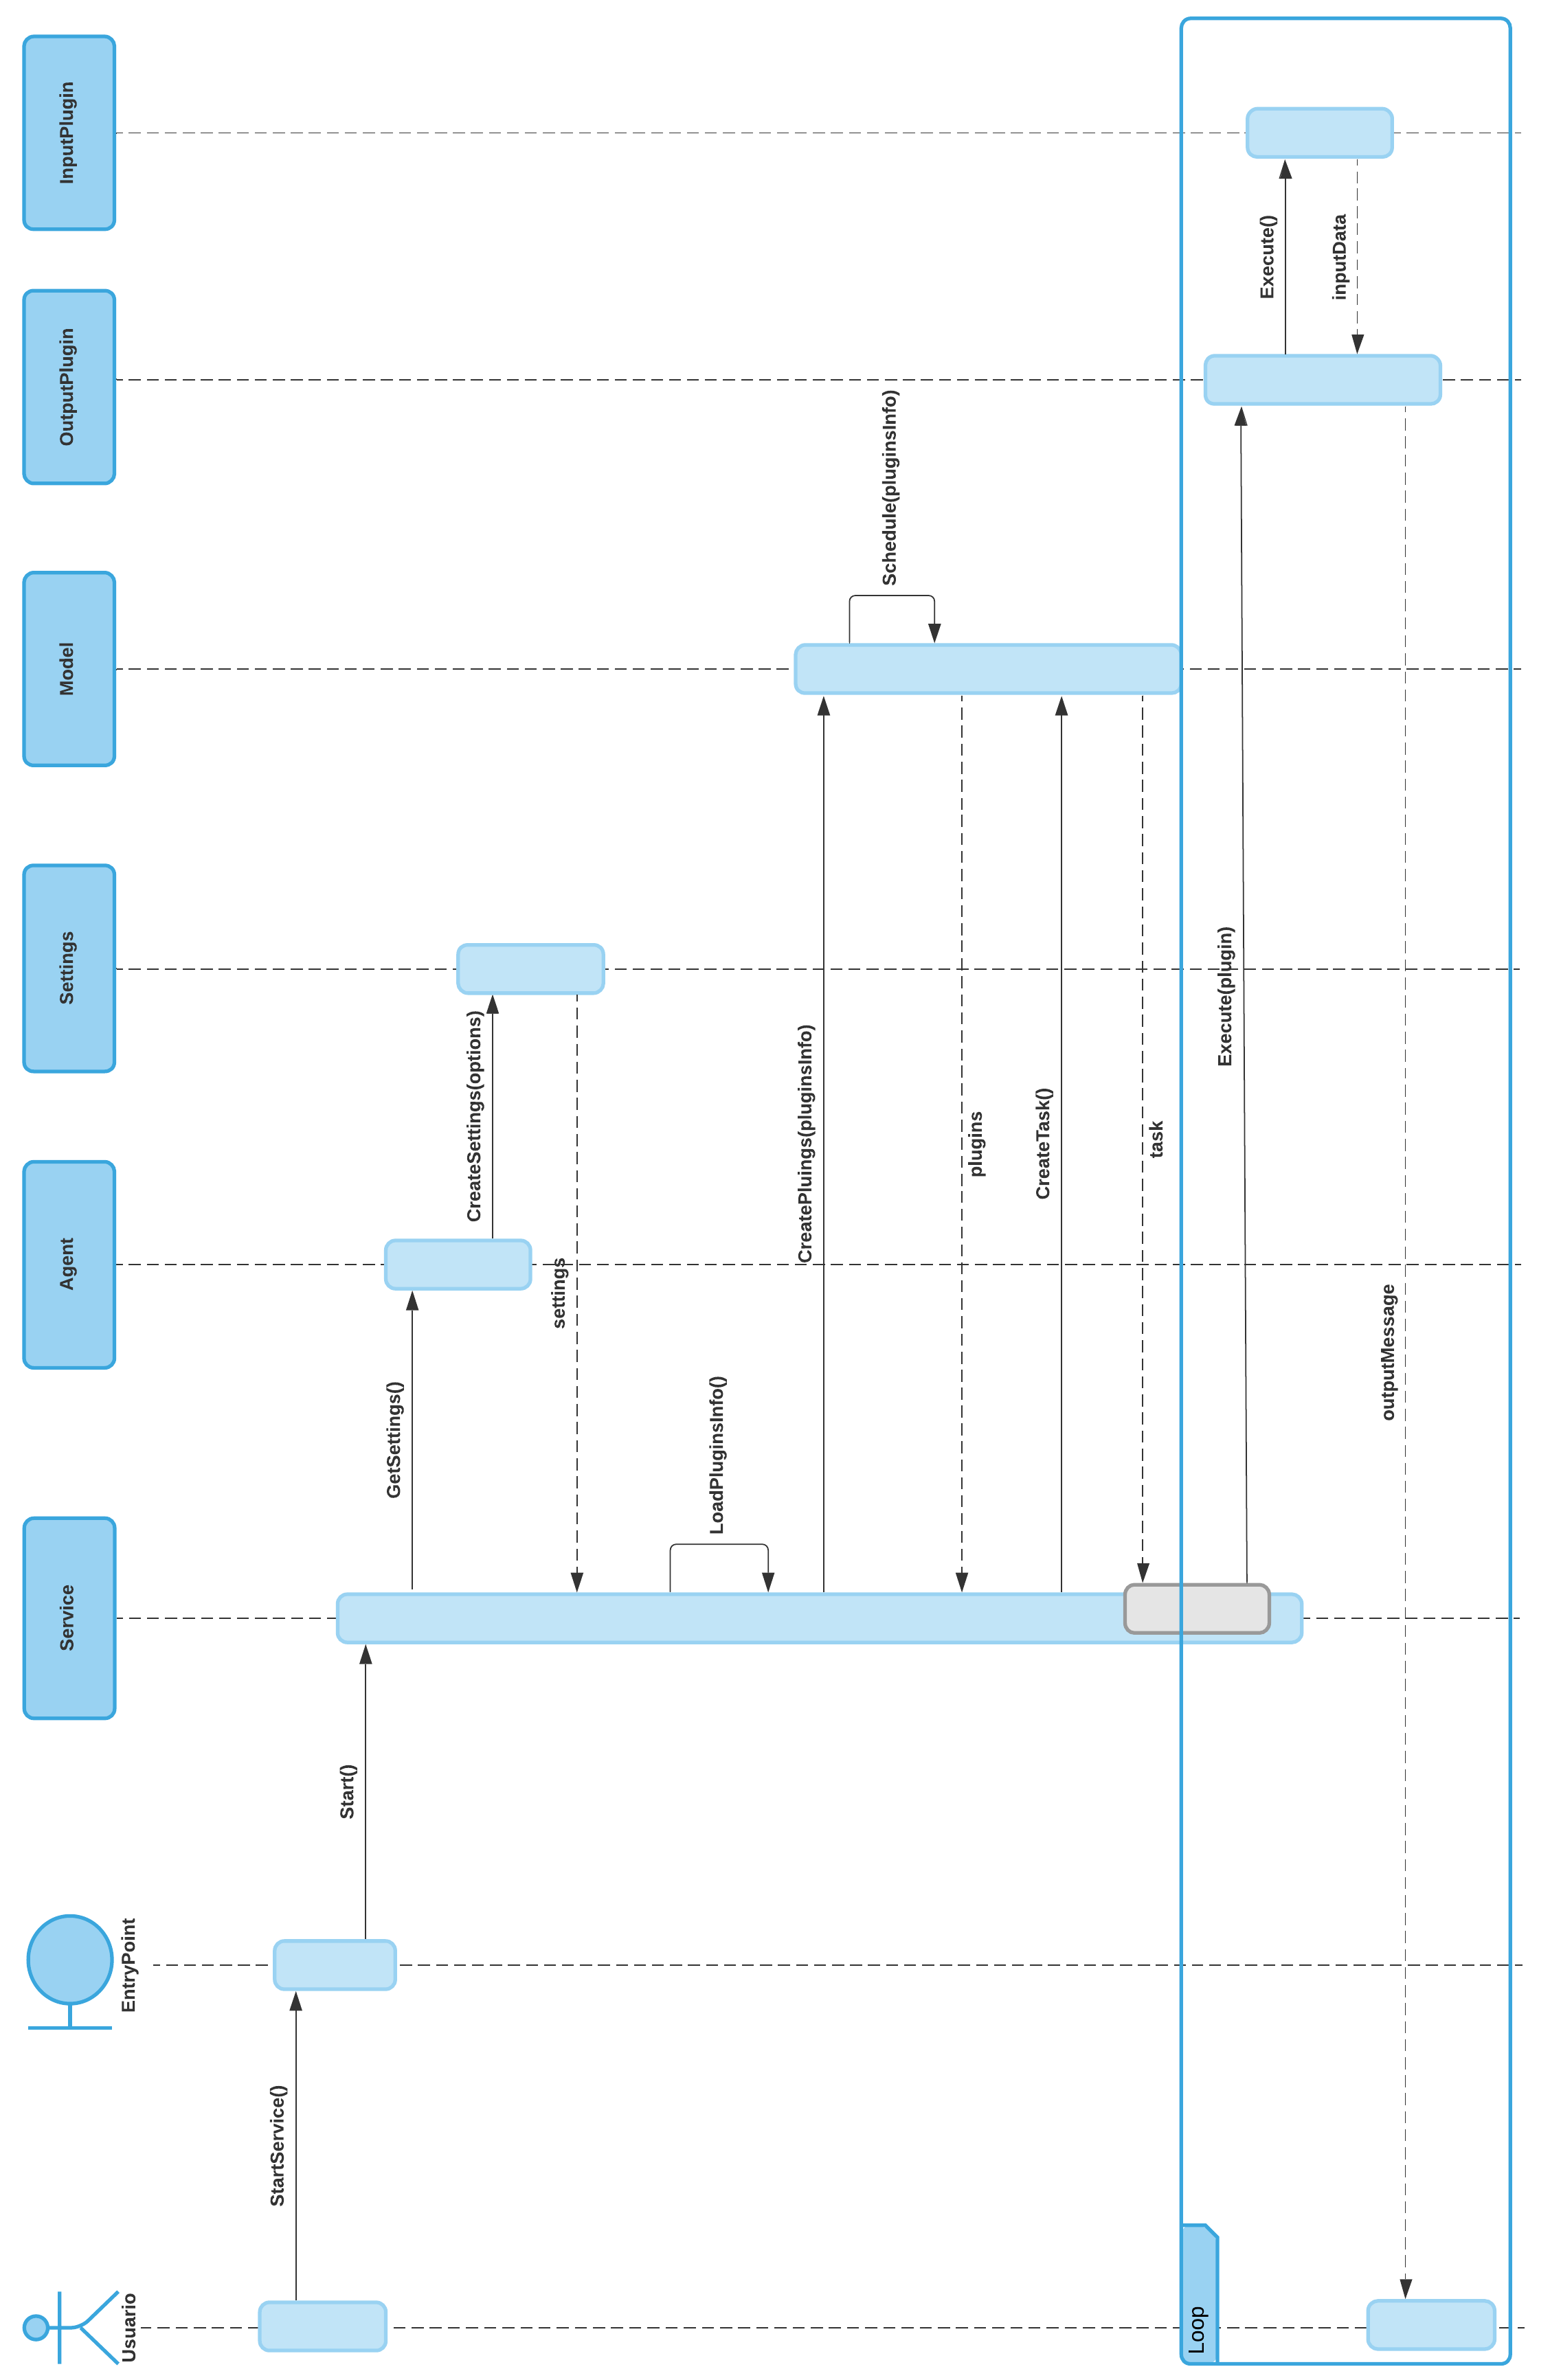
\includegraphics[scale=0.25]{diagrama-secuencia-servicio.png}
        \caption{Diagrama de secuencia - Servicio}
        \label{fig:sequence-diagram-service}
    \end{figure}
    
    \begin{figure}[h!]
    \centering
        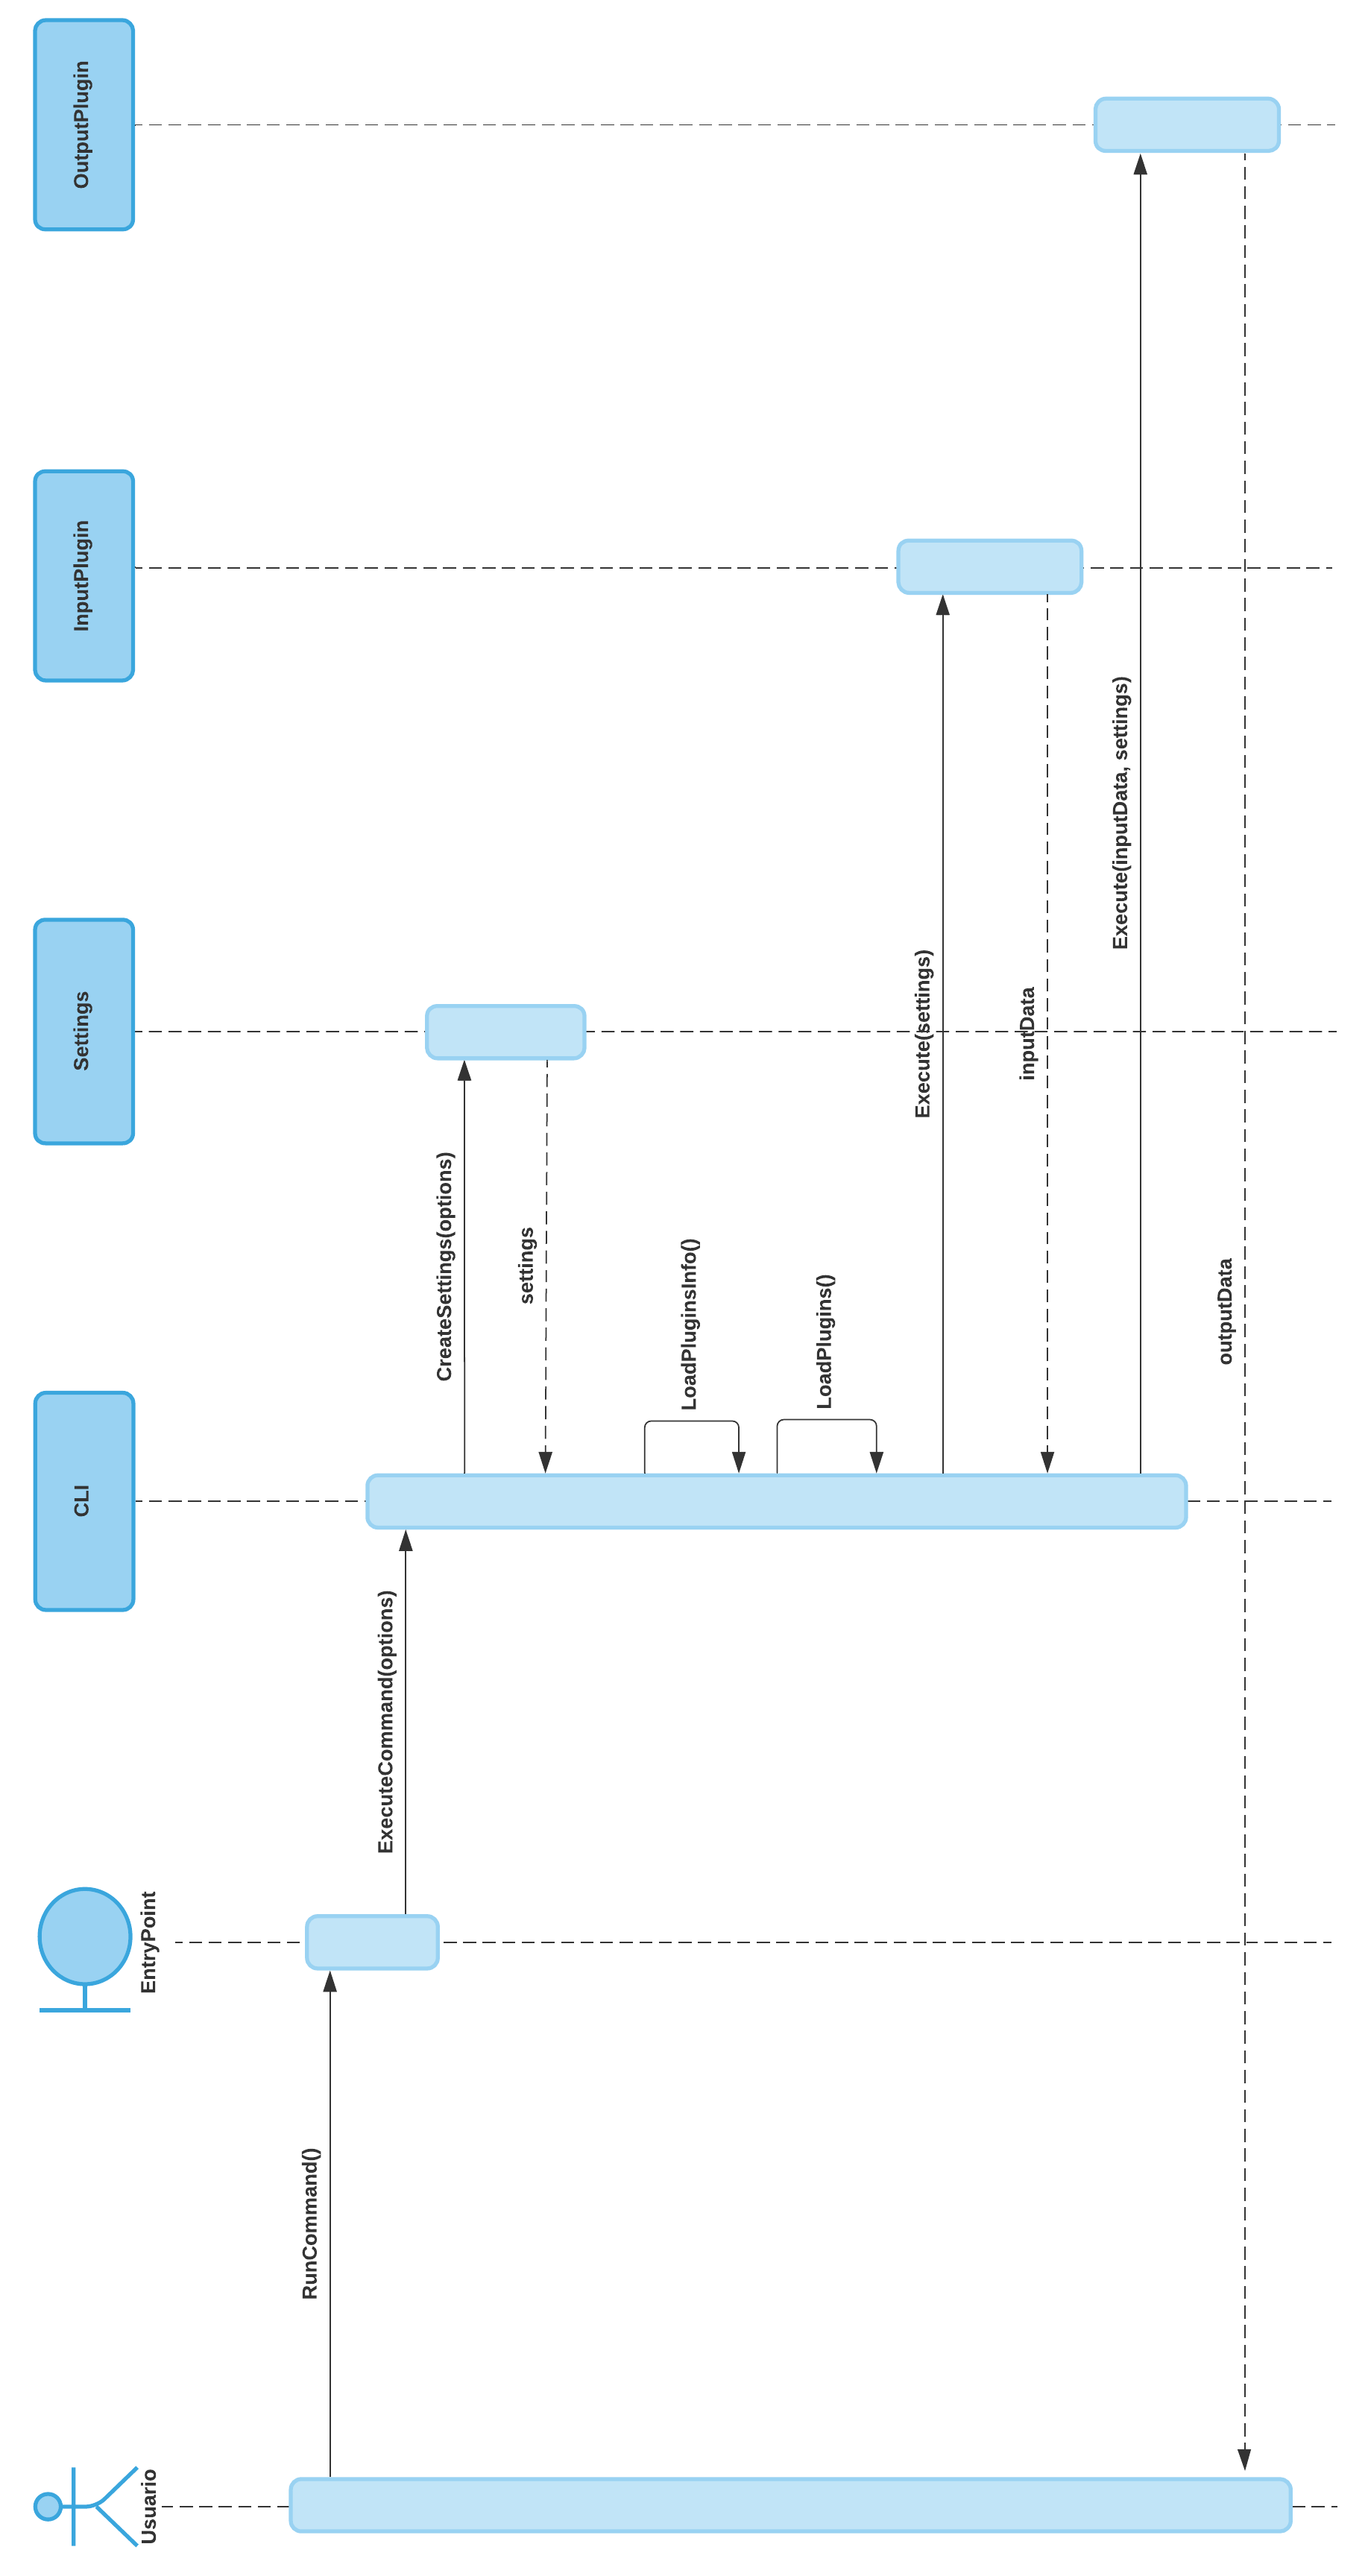
\includegraphics[scale=0.25]{diagrama-secuencia-cli.png}
        \caption{Diagrama de secuencia - \textit{CLI}}
        \label{fig:sequence-diagram-cli}
    \end{figure}
    